% !TEX encoding = UTF-8 Unicode
\documentclass{../headers/td_upc}
\input{../headers/header_td.tex}

\def\version{eno}
%\def\version{cor}

\usepackage{hyperref}
\ue{MV4AE035}

\providecommand{\T}{\mathbb{T}}
\providecommand{\1}{\mathds{1}}
\title{TD 1 : Régression linéaire simple}


\newcommand{\miniscule}{\@setfontsize\miniscule{5}{6}}
%-----------------------------------------------------------------------------
\begin{document}
	\maketitle
	
	\exo{Rappels de cours}
	
	\begin{enumerate}
		\item Rappeler le principe d'une régression linéaire simple. Préciser les hypothèses.
		\item Rappeler les définitions des quantités suivantes :
		$x_i$, $y_i$, $\beta_0$, $\beta_1$, $\bar x$, $\bar y$, $\hat \beta_0$, $\hat \beta_1$, $\epsilon_i$, $\hat \epsilon_i$.
		On indiquera en particulier si ces quantités sont déterministes ou aléatoires.
		\item Faire un schéma pour donner une interprétation géométrique à la régression linéaire simple.
		\item Donner la définition du coefficient de détermination $R^2$ et son interprétation. Montrer que ce coefficient s'écrit
		\[
		R^2 = \dfrac{[\sum_{i=1}^n (x_i - \bar x)(y_i - \bar y)]^2}{\sum_{i=1}^n (x_i - \bar x)^2 \sum_{i=1}^n(y_i - \bar y)^2} =: \dfrac{s_{x y}^4}{s_{x}^2 s_{y}^2} = \rho(x, y)^2\,.
		\]
		où $\rho(x,y)$ est le coefficient de corrélation empirique entre $x$ et $y$.
		\cor{
		Par définition :
		\[
		R^2 = 1 - \frac{RSS}{TSS} = \frac{ESS}{TSS} 
		= \frac{\|\hat{\mathbf{y}} - \bar{y}\mathbf{1}\|^2}{\|\mathbf{y} - \bar{y}\mathbf{1}\|^2}
		\]
		Mais :
		\[
		\|\hat{\mathbf{y}} - \bar{y}\mathbf{1}\|^2
		= \sum_i (\hat y_i - \bar y)^2
		= \sum_i (\hat \beta_0 + \hat \beta_1 x_i - \bar y)^2
		= \sum_i (\bar y - \hat \beta_1 \bar x + \hat \beta_1 x_i - \bar y)^2
		=  \hat \beta_1^2 \sum_i (x_i - \bar x)^2
		\]
		et :
		\[
		\|\mathbf{y} - \bar{y}\mathbf{1}\|^2
		= \sum_i (y_i - \bar y)^2
		\]
		Donc :
		\[
		R^2
		= \frac{\hat \beta_1^2 \sum_i (x_i - \bar x)^2}{\sum_i (y_i - \bar y)^2}
		= \frac{[\sum_{i=1}^n (x_i - \bar x)(y_i - \bar y)]^2 \sum_i (x_i - \bar x)^2}{[\sum_i (x_i - \bar x)^2]^2 \sum_i (y_i - \bar y)^2}
		= \frac{[\sum_{i=1}^n (x_i - \bar x)(y_i - \bar y)]^2}{\sum_i (x_i - \bar x)^2 \sum_i (y_i - \bar y)^2}
		\]
		}
		\item Donner les hypothèses supplémentaires dans le cas d'une régression linéaire gaussienne.
		Quelles informations a-t-on en plus dans ce contexte ?
	\end{enumerate}
	
	\cor{\newpage}
	
	\exo{}
	L'étude statistique ci-dessous porte sur les poids (en kg) respectifs des pères $p_{i}$,
	et ceux de leurs fils aînés $f_{i}$ avec $i=1,\cdots,12$.
	Les résultats sont tracés sur le graphique suivant
	
	\begin{center}
		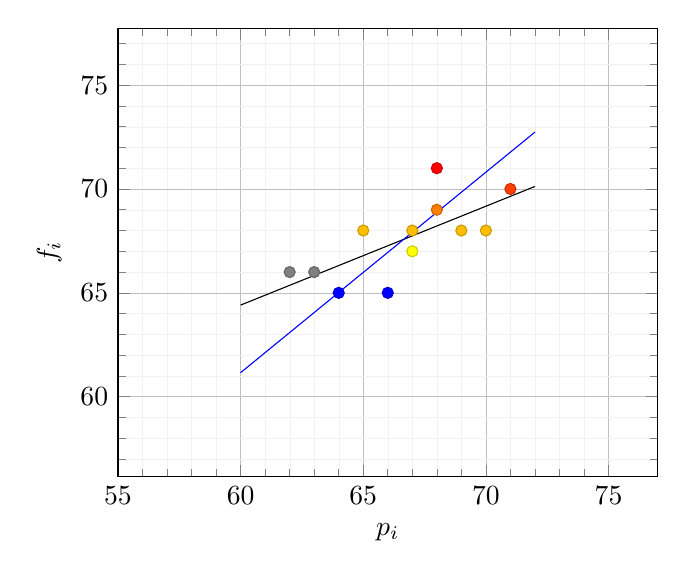
\begin{tikzpicture}
			\begin{axis}[grid=both,%
				grid style={line width=.1pt, draw=gray!10},
				major grid style={line width=.2pt,draw=gray!50},
				minor tick num=4,
				enlargelimits={abs=5},
				xlabel=$p_i$,
				ylabel=$f_i$,
				]
				\addplot[blue,scatter,only marks]%
				table[] {
					x     y  
					65    68 
					63    66 
					67    68 
					64    65 
					68    69 
					62    66 
					70    68 
					66    65 
					68   71  
					67   67  
					69   68  
					71   70  
				};
				\addplot[domain=60:72]{35.85 + 0.476*x};
				\addplot[blue, domain=60:72]{3.258 + 0.965*x};
			\end{axis}
		\end{tikzpicture}
	\end{center}
	
	%\[
	%\begin{array}{ccccccccccccc}
	%p_{i} & 65 & 63 & 67 & 64 & 68 & 62 & 70 & 66 & 68 & 67 & 69 & 71 \\
	%f_{i} & 68 & 66 & 68 & 65 & 69 & 66 & 68 & 65 & 71 & 67 & 68 & 70
	%\end{array}
	%\]
	% x <- c(65, 63, 67, 64, 68, 62, 70, 66, 68, 67, 69, 71)
	% y <- c(68, 66, 68, 65, 69, 66, 68, 65, 71, 67, 68, 70)
	% lm(y ~ x)
	% lm(x ~ y)
	On donne quelques résultats numériques :
	$$
	\sum p_{i}=800, \sum p_{i}^{2}=53418, \sum p_{i} f_{i}=54107, \sum f_{i}=811, \sum f_{i}^{2}=54849
	$$
	\begin{enumerate}
		\item  Calculer la droite des moindres carrés du poids des fils en fonction du poids des pères.
		\cor{
		\[
		\hat \beta_1 
		= \frac{\sum_{i=1}^n (f_i - \bar{f})(p_i - \bar{p})}{\sum_{i=1}^n (p_i - \bar{p})^2}
		= \frac{\sum_{i = 1}^n f_ip_i - \frac{1}{n}(\sum_{i = 1}^np_i)(\sum_{i = 1}^nf_i)}{\sum_{i=1}^n p_i^2 - \frac{1}{n}(\sum_{i=1}^n p_i)^2}
		= \frac{54107 - 800 \times 811 / 12}{53418 - 800^2/12}
		= 0.476378
		\]
		\[
		\hat\beta_0 = \bar{f} - \hat\beta_1 \bar{p} = 811 / 12 - 0.476378 \times 800 / 12 = 35.8248
		\]
		}
		\item  Calculer la droite des moindres carrés du poids des pères en fonction du poids des fils.
				\cor{
		\[
		\hat \beta_1 
		= \frac{\sum_{i=1}^n (f_i - \bar{f})(p_i - \bar{p})}{\sum_{i=1}^n (f_i - \bar{f})^2}
		= \frac{\sum_{i = 1}^n f_ip_i - \frac{1}{n}(\sum_{i = 1}^np_i)(\sum_{i = 1}^nf_i)}{\sum_{i=1}^n f_i^2 - \frac{1}{n}(\sum_{i=1}^n f_i)^2}
		= \frac{54107 - 800 \times 811 / 12}{54849 - 811^2/12}
		= 1.036403
		\]
		\[
		\hat\beta_0 = \bar{p} - \hat\beta_1 \bar{f} = 800 / 12 - 0.476378 \times 811 / 12 = -3.376903
		\]
		}
		\item  Les deux droites de régression sont-elles identiques ? Identifiez-les sur le graphique.
		\cor{
		La droite grise correspond à la régression des fils par rapport aux pères.
		}
		\item  En quel point se coupent ces deux droites ? Que vaut le produit des pentes des deux droites ?
		\cor{
		Les deux droites passent par le point $(\bar{p}, \bar{f})$ = $(66.66667, 67.58333)$.
		Le produit des deux pentes est égal au $R^2$.
		}
		\item  Estimer $\sigma^{2}$ dans le premier modèle de régression.
		Un père pèse $70$ kilos, peut-il raisonnablement espérer que son fils aîné en pèse $80$ ?
		% On donne le quantile à $0.975$ de la loi de Student à $10$ degrés de libertés : 
		% $q_{t, 10}(0.975) = 2.228139$.
		\cor{
		\begin{align*}
		\hat{\sigma}^2 
		&= \frac{1}{n-2}\sum_{i = 1}^n (f_i - \hat f_i)^2
		= \frac{1}{n-2} (1 - R^2) \sum_i(f_i - \bar f)^2\\
		&= 1 / 10 * (1 - 1.036403 \times 0.476378) \times (54849 - 811^2/12)
		= 1.970275
		\end{align*}
		Prédiction :
		\[
		\hat f_{n+1} 
		= \hat \beta_0 + \hat \beta_1 p_{n+1}
		= 35.8248 + 0.476378 \times 70
		= 69.17126
		\]
		Variance estimée :
		\begin{align*}
		\hat \sigma^2_{n+1} 
		&= \hat{\sigma}^2 \left(1 + \frac{1}{n} + \frac{1}{\sum_{i=1}^n (p_i - \bar{p})^2} (p_{n+1} - \bar{p})^2\right)
		\\
		&= 1.970275 \times (1 + 1/12 + (70 - 800 / 12)^2 / (53418 - 800^2/12))
		= 2.393031
		\end{align*}
		Si on supppose qu'approximativement :
		\[
		f_{n+1} \sim \mathcal{N}(\hat f_{n+1}, \hat \sigma^2_{n+1}) 
		\]
		Alors 
		\[
		\mathbb{P}[f_{n+1} \geq 80] \approx 1.278977e^{-12}
		\]
		Il est très peu probable que le fils de cet homme fasse $80kg$.
		
		\textbf{Note}: pour faire les choses de manière rigoureuse, il faut faire un test de Student (voir exercice suivant).
		
% 		Sous l'hypothèse gaussienne : 
% 		\[
%     \frac{f_{n+1} - \hat{f}_{n+1}}{\sqrt{\hat{\sigma}^2 \left(1 + \frac{1}{n} + \frac{1}{ns_{p}^2} (p_{n+1} - \bar{p})^2\right)}}
%     \sim
%     \mathcal{T}_{n-2}
% 		\]
% 		Donc l'intervalle de prédiction à $95\%$ est :
% 		\[
% 		[69.17126 - 2.228139 \times \sqrt{2.393031} ; 73.93504 + 2.228139  \times \sqrt{6.271525}]
% 		=
% 		[65.72446 ; 72.61806]
% 		\]
% 		Il est peut probable que le fils de cet homme fasse $80kg$.
		}
	\end{enumerate}
	
	
	\cor{\newpage}
	
	\exo{}
	Dans de nombreux cas, 
	lorsque l'on étudie le lien entre $Y$ et $X$ nous savons que si $X=0$, alors $Y=0$. 
	On peut alors simplifier le modèle linéaire en cherchant juste à ajuster 
	les points sur une droite d'ordonnée à l'origine nulle. 
	On étudie la régression linéaire 
	$y_{i}=\beta x_{i}+\varepsilon_{i},$ où les $\varepsilon_{i}$ sont centrées,
	non corrélées et de même variance $\sigma^{2}$. 
	\begin{enumerate}
	  \item Montrez que l'estimateur des moindres carrés s'écrit dans ce cas :
	  \[
	  \hat{\beta}=\frac{\sum_{i=1}^{n} x_{i} y_{i}}{\sum_{i=1}^{n} x_{i}^{2}}
	  \]
	  \cor{
		L'estimateur des moindres carrés est par définition :
		\[
		\hat\beta = \mbox{argmin}_{\beta} \sum_{i=1}^n(y_i - \beta x_i)^2
		\]
		On trouve l'expression en dérivant la fonction à une seule variable.
		}
		\item Une autre manière de construire un estimateur est de trouver la droite
		qui passe à la fois par l'origine et par le point de gravité $(\bar{x}, \bar y)$.
		Montrez qu'alors l'estimateur de la pente s'écrit :
		\[
	  \tilde{\beta}=\frac{\sum_{i=1}^{n} y_{i}}{\sum_{i=1}^{n} x_{i}}
	  \]
		\cor{
		La droite qui passe par l'origine et par le point $(\bar{x}, \bar y)$ est 
		telle que
		\(
		\bar y = \tilde \beta \bar x
		\),
		ce qui donne l'expression attendue.
		}
		\item   Montrer que $\hat{\beta}$ et $\tilde{\beta}$ sont des estimateurs non biaisés de $\beta$.
		\cor{
		On remplace $y_i$ par $\beta x_i + \epsilon_i$ dans chacun des deux estimateurs :
		\[
				\hat\beta 
				= \frac{\sum_{i=1}^{n} x_{i} (\beta x_i + \epsilon_i)}{\sum_{i=1}^{n} x_{i}^{2}}
				= \beta + \frac{\sum_{i=1}^{n} x_{i} \epsilon_i}{\sum_{i=1}^{n} x_{i}^{2}}
		\]
		\[
				\tilde\beta 
				= \frac{\sum_{i=1}^{n} \beta x_i + \epsilon_i}{\sum_{i=1}^{n} x_{i}}
				= \beta + \frac{\sum_{i=1}^{n} \epsilon_i}{\sum_{i=1}^{n} x_{i}}
		\]
		Comme $\mathbb{E}[\epsilon_i] = 0$, on trouve bien que les deux estimateurs sont non biaisés.
		}
		\item   Montrer que la variance de $\tilde{\beta}$ est strictement plus grande que la variance de
		$\hat{\beta},$ sauf dans le cas où les $x_{i}$ sont tous égaux. (On pourra utiliser l'inégalité de Cauchy-Schwarz.)
		Ce résultat était-il prévisible ?
		\cor{
		Comme les $\epsilon_i$ sont non corrélés et de variance $\sigma^2$, 
		on obtient grâce aux expressions précédentes :
		\[
		\mathbb{V}[\hat\beta] 
		= \frac{\sum_{i=1}^{n} x_{i}^2\sigma^2}{[\sum_{i=1}^{n} x_{i}^{2}]^2}
		= \frac{\sigma^2}{\sum_{i=1}^{n} x_{i}^{2}}
		\]
		et
		\[
		\mathbb{V}[\tilde\beta] 
		= n\frac{\sigma^2}{[\sum_{i=1}^{n} x_{i}]^{2}}
		\]
		Par l'inégalité de Cauchy-Schwarz :
		\[
		\left(\sum_{i=1}^{n} x_{i}\right)^2
		= \left(\sum_{i=1}^{n} x_{i} \times 1\right)^2
		\leq \left(\sum_{i=1}^{n} x_{i}^2\right) \left(\sum_{i=1}^{n} 1^2\right)
		= n \left(\sum_{i=1}^{n} x_{i}^2\right)
		\]
		avec égalité ssi tous les $x_i$ sont égaux.
		D'où l'inégalité des variances voulue.
		Ceci est cohérent avec le théorème de Gauss-Markov.
		}
		\item Redémontrer le théorème de Gauss-Markov dans ce cas particulier.
		\cor{
		On utilise la même démarche que dans le cours, et on peut conclure par
		l'inégalité de Cauchy-Schwarz :
		\[
		1 = \left(\sum_{i=1}^{n} q_i x_{i}\right)^2
		\leq \left(\sum_{i=1}^{n} x_{i}^2\right) \left(\sum_{i=1}^{n} q_i^2\right).
		\]
		}
	\end{enumerate}
	
	
	\cor{\newpage}
	
	\exo{}
	On suppose que le modèle de régression linéaire simple de $Y$ en fonction de $X$, 
	avec des erreurs centrées et non corrélées, est valide :
	\[
	Y=\beta_{0} + \beta_{1} X + \varepsilon\,.
	\]
	Montrer qu'alors il en est de même pour le modèle de régression linéaire de $X$ en fonction de $Y$. 
	Quels sont les paramètres de ce modèle ?
	
	\cor{
	On obtient le modèle suivant :
	\[
	X 
	= - \frac{\beta_0}{\beta_1} + \frac{1}{\beta_1} Y - \frac{1}{\beta_1} \epsilon
	= \beta_0' + \beta_1' Y + \epsilon'
	\]
	avec :
	\[
	\beta_0' = - \frac{\beta_0}{\beta_1}
	\quad
	\beta_1' = \frac{1}{\beta_1}
	\quad
	(\sigma')^2 = \frac{\sigma^2}{\beta_1^2}
	\]
	}
	
	\cor{\newpage}
	
	\exo{}
	On considère un produit dont le coût de fabrication est $x_{0}$. 
	Supposons que le nombre de produits vendus en une semaine, 
	$y$ dépend du prix de vente $x$ selon un modèle linéaire simple.
	\begin{enumerate}
		\item  Quel est le prix de vente maximisant la marge de l'entreprise ?
		\cor{
		Par hypothèse, on a :
		\[
		y = \beta_0 + \beta_1 x
		\]
		On peut supposer que $\beta_1 < 0$, car plus un produit est cher, moins il se vend.
		On suppose également que $\beta_0 > 0$, un produit de prix nul continuant de se vendre.
		La marge est le nombre d'unités vendues, multiplié par le prix de vente moins le prix de revient :
		\[
		m(x) = y (x - x_0) = (\beta_0 + \beta_1 x)(x - x_0)
		\]
		C'est un polynôme de degré 2. Si $\beta_1 < 0$, il admet un unique maximum $x_m$ tel que :
		\[
		m'(x_m) = 2 \beta_1 x_m + \beta_0 - \beta_1 x_0 = 0
		\quad \mbox{ie} \quad
		x_m = \frac{\beta_1 x_0 - \beta_0}{2 \beta_1}
		\]
		ce prix est bien positif, car $\beta_0 - \beta_1 x_0 > 0$.
		}
		\item  Sur les trois dernières semaines, un industriel a fait varier le prix du produit. 
		On dispose des données suivantes.
		\[
		\begin{array}[]{cccc}
			\hline
			\text{prix} & 113 & 115 & 120 \\
			\text{quantité} & 230 & 200 & 125 \\
			\hline
		\end{array}
		\]
		Sachant que le coût de fabrication est de $100$ euros, quel prix de vente lui conseillez-vous~?
		\cor{
		On commence par ajuster la régression :
		\[
		\hat{\beta_1} 
		= \frac{\sum_{i = 1}^n y_ix_i - \frac{1}{n}(\sum_{i = 1}^nx_i)(\sum_{i = 1}^ny_i)}{\sum_{i=1}^n x_i^2 - \frac{1}{n}(\sum_{i=1}^n x_i)^2}
		= -15
		\]
		et
		\[
		\hat\beta_0 = \bar y - \hat \beta_1 \bar x = 1925
		\]
		On estime donc le prix de vente optimal par :
		\[
		\hat x_m 
		= \frac{\hat \beta_1 x_0 - \hat\beta_0}{2 \hat\beta_1}
		= \frac{-15 * 100 - 1925}{2 \times -15}
		= 114.1667
		\]
		}
	\end{enumerate}
	
	
	\cor{\newpage}
	
	\exo{\!\!\!\!*} 
	Soit $y_{1}, \ldots, y_{n}$ des réels. Pour mesurer l'écart d'un réel $x$ 
	à l'ensemble des $y_{i},$ on peut utiliser la distance 
	$D(x)=\sum_{i=1}^{n} f\left(y_{i}-x\right)$ où $f$ est une fonction positive,
	paire, s'annulant en 0, continue et croissante sur les réels positifs.
	\begin{enumerate}
		\item Montrer que le réel qui minimise cette distance lorsque $f(t)=t^{2}$ est la moyenne des $y_{i}$.
		\cor{
		Dans ce cas, $D$ est une fonction quadratique, qui admet un unique minimum en son point critique,
		et :
		\[
		D'(\hat \beta_0) = 2 \sum_i (y_i - \hat\beta_0) = 0
		\quad \mbox{donc}\quad
		\hat\beta_0 = \frac{1}{n}\sum_i y_i.
		\]
		}
		\item On suppose maintenant que $f(t)=\abs{t}$. 
		Montrer que le réel qui minimise la distance $D(x)$ est la médiane des $y_{i}$.
		
		{\it Indication : considérer que $y_{1} \leq$ $\cdots \leq y_{n}$, 
		réécrire $D(x)$ sur l'intervalle $[y_{j}, y_{j+1}[$, puis tracer $D(x)$.
		On traitera le cas où $n=2 p+1,$ puis le cas où $n=2 p$}.
		
		\cor{
		Pour $y_j \leq x < y_{j+1}$, on a :
		\[
		D(x) 
		= - \sum_{i=1}^j (y_i - x) + \sum_{i=j+1}^n (y_i - x)
		= - \sum_{i=1}^j y_i + \sum_{i=j+1}^n y_i + (2j - n) x
		\]
		Si $n = 2 p + 1$, la pente est négative pour $j \leq p$, puis positive pour $j \geq p+1$.
		Le minimum est alors atteint en $y_{p+1}$, qui est bien la médiane par définition.
		
		Si $n = 2p$, la pente est négative pour $j \leq p-1$, nulle pour $j = p$, puis positive pour $j \geq p$.
		La fonction est constante entre $y_p$ et $y_{p+1}$ et vaut sa valeur minimale.
		Elle est donc bien minimisé en la médiane $(y_p + y_{p+1})/2$.
		}
		
		\item Soient $w_{1}, \ldots, w_{n}$ des poids positifs tels que $\sum_{i=1}^n w_i = 1$.
		Quel est le réel qui minimise la distance 
		\(
		D(x) = \sum_{i=1}^n w_i (y_i - x)^2
		\) ?
		\cor{
		En annulant la dérivée 
		$D'(x) = -2 \sum_{i=1}^n w_i (y_i - x)$,
		on trouve que le minimiseur est la moyenne pondérée $\sum_{i=1}^n w_i y_i$.
		}
		\item On définit la médiane pondérée des $y_i$ comme l'élément $y_k$ tel que
		\(
		\sum_{i=1}^{k-1} w_i \leq \frac{1}{2}
		\)
		et
		\(
		\sum_{i=k+1}^n w_i \leq \frac{1}{2}.
		\)
		Montrez que la médiane pondérée est le réel qui minimise la distance\;:
		\(
		D(x) = \sum_{i=1}^n w_i |y_i - x|
		\).
		\cor{
		La preuve est similaire au cas précédent, mais en utilisant les poids.
		}
	\end{enumerate}
	
	\cor{\newpage}
	
	\exo{\!\!\!\!\!\!\!\!*}
	Soit $y_{1}, \ldots, y_{n}$ et $x_{1}, \ldots, x_{n}$ des réels. 
	Dans le modèle linéaire simple $y_{i}=\beta_{0}+\beta_{1} x_{i}+\varepsilon_{i}$, 
	on considère la somme des erreurs en valeur absolue
	\[
	S\left(\beta_{1}, \beta_{2}\right)=\sum_{i=1}^{n}\abs{y_{i}-\beta_{0}-\beta_{1} x_{i}}\,.
	\]
	et on notera $\tilde{\beta}_{0}$ et $\tilde{\beta}_{1}$ les estimateurs des moindres valeurs absolues, 
	\textit{i.e.} les valeurs de $\beta_{0}$ et $\beta_{1}$ minimisant la fonction $S(\cdot, \cdot)$. 
	On cherche une stratégie pour obtenir $\tilde{\beta}_{0}$ et $\tilde{\beta}_{1}$.
	\begin{enumerate}
		\item La valeur de $\beta_{1}$ étant fixée, quelle est la valeur de $\beta_{0}$ qui minimise la fonction 
		$g\left(\beta_{0}\right)=\sum_{i=1}^{n}\left|y_{i}-\beta_{0}-\beta_{1} x_{i}\right|$ ?
		\cor{
		Si $\beta_1$ est fixé, la fonction :
		\(
		g\left(\beta_{0}\right) = \sum_i | y_i - \beta_1 x_i - \beta_0 |
		\)
		est minimisée en $\tilde \beta_0 = \mbox{med}(\mathbf{y} - \beta_1 \mathbf{x})$ d'après l'exercice précédent.
		}
		\item En déduire un algorithme pour obtenir $\tilde{\beta}_{0}$ et $\tilde{\beta}_{1}$.
		\cor{
		On initialise $\beta_1^0$ à une valeur quelconque, par exemple l'estimateur des moindres carrés.
		On procède ensuite de maniière itérative :
		\begin{align*}
		\beta_0^{k+1} &= \mbox{med}(y_i - \beta_1^{k} x_i)\\
		\beta_1^{k+1} &= \mbox{med}(\frac{y_i - \beta_0^{k+1}}{x_i}; w_i)
		\end{align*}
		où la seconde médiane est pondérée par les $w_i = \frac{|x_i|}{\sum_{j=1}^n |x_j|}$.
		}
	\end{enumerate}
	
	
	\cor{\newpage}
	
%	\exo{}
%	Montrer que le coefficient de détermination $R^{2}$ est égal au carré du coefficient de corrélation empirique entre les $x_{i}$ et les $y_{i}$ défini par
%	\[
%	\rho(x, y)=\frac{s_{x y}}{s_{x} s_{y}}=\frac{\sum_{i=1}^{n}\left(x_{i}-\bar{x}\right)\left(y_{i}-\bar{y}\right)}{\sqrt{\sum_{i=1}^{n}\left(x_{i}-\bar{x}\right)^{2} \sum_{i=1}^{n}\left(y_{i}-\bar{y}\right)^{2}}}
%	\]
%	
%	\cor{\newpage}
	
	
	\exo{Retour sur le cas gaussien}
	
	Dans le modèle linéaire simple, si on considère la normalité des $\varepsilon_{i},$ alors
	\[
	y_{i} \sim \mathcal{N}\left(\beta_{0}+\beta_{1} x_{i}, \sigma^{2}\right)\,, \quad i=1, \ldots, n\,.
	\]
	\begin{enumerate}
		\item  Exprimer la vraisemblance $L\left(\beta_{0}, \beta_{1}, \sigma^{2}\right)$ des observations.
		\item  Quelles sont les valeurs de $\beta_{0}$ et $\beta_{1}$ maximisant cette vraisemblance ?
		\item  Quelle est la valeur de $\sigma^{2}$ maximisant cette vraisemblance ? 
		Que peut-on alors dire de l'estimateur du maximum de vraisemblance de $\sigma^{2}$ ?
	\end{enumerate}
	
	\cor{\newpage}
	
	\exo{Fréquence Cardiaque}
	On s'intéresse à la fréquence cardiaque de sportifs amateurs mesurée après
	trois quarts d'heure d'un effort soutenu.
	On veut déterminer si l'âge du sportif a une influence sur sa fréquence cardiaque
	après un effort soutenu. On dispose de $n = 40$ observations du couple 
	$(y_i;x_i)$ où $y_i$ est la fréquence cardiaque et $x_i$ l'âge du
	sportif $i$.
	On suppose un modèle linéaire gaussien classique entre $y$ et $x$,
	d'intercept $\beta_0$ et de pente $\beta_1$.
	On donne :
	\[
	\bar y = 171.3
	~ ; ~
	\bar x = 38.4
	~ ; ~
	\sum_{i=1}^{40} (x_i - \bar x)^2 = 4381
	~ ; ~
	\sum_{i=1}^{40} (y_i - \bar y)^2 = 424
	~ ; ~
	\sum_{i=1}^{40} (x_i - \bar x)(y_i - \bar y) = -961
	\]
	\begin{enumerate}
	\item Donnez l'expression de $\hat \beta_0$ et $\hat \beta_1$, et calculez leur valeur.
	\cor{
	\[
	\hat \beta_1 
	= \frac{s^2_{x,y}}{s^2_x} 
	= \frac{\sum_{i=1}^{40} (x_i - \bar x)(y_i - \bar y)}{\sum_{i=1}^{40} (x_i - \bar x)^2}
	= \frac{-961}{4381}
	= -0.2193563
	\]
	\[
	\hat\beta_0 
	= \bar y - \hat \beta_1 \bar x
	= 171.3 - (-0.2193563) \times 38.4
	= 179.7233
	\]
	}
	\item Calculez le coefficient de détermination $R^2$. Interprétez.
	\cor{
	\begin{align*}
	R^2 = \rho(x, y)^2 
	= \frac{[\sum_{i=1}^n (x_i - \bar x)(y_i - \bar y)]^2}{\sum_{i=1}^n (x_i - \bar x)^2 \sum_{i=1}^n(y_i - \bar y)^2}
	= \frac{(-961)^2}{4381 \times 424}
	= 0.4971731
	\end{align*}
	La régression n'explique qu'envirion $50\%$ de la variance.
	}
	\item Donnez la loi de $\hat \beta_1$ en fonction de $\sigma^2$.
	\cor{
	\[
	\hat \beta_1 \sim \mathcal{N}\left(\beta_1, \frac{\sigma^2}{\sum_{i=1}^n (x_i - \bar x)^2}\right)
	\]
	}
	\item Donnez la définition de $\hat y_i$ et $\hat \epsilon_i$.
	Que représente cette quantité ? On donne :
	\[
	\sum_{i=1}^n (y_i - \hat y_i)^2 = 213.3.
	\]
	En déduire un estimateur $\hat\sigma^2$ sans bias pour la variance, 
	puis un estimateur $\hat\sigma^2_1$ pour la variance de $\hat\beta_1$.
	\cor{
	\[
	\hat y_i = \hat\beta_0 + \hat\beta_1 x_i \quad \hat \epsilon_i = y_i - \hat y_i
	\]
	$\hat \epsilon_i$ sont les résidus réalisés.
	\[
	\hat{\sigma}^2 
	= \frac{1}{n-2} \sum_{i=1}^n (y_i - \hat y_i)^2
	= \frac{1}{38} 213.3
	= 5.613158.
	\]
	Un estimateur pour la variance de $\hat\beta_1$ est donné par :
	\[
	\hat\sigma^2_1 
	= \frac{\hat{\sigma}^2}{\sum_{i=1}^n (x_i - \bar x)^2}
	= \frac{5.613158}{4381}
	= 0.00128125.
	\]
	}
	\item Testez l'hypothèse $H_0: \beta_1 = 0$ v.s. $H_1: \beta_1 \neq 0$.
	On donne le quantile de la loi de Student à $38$ degrés de libertés à $97.5\%$:
	$q_{t,38}(97.5\%) = 2.024394$. Interprétez.
	\cor{
	On a :
	\[
	\frac{\beta_1 - \hat\beta_1}{\sqrt{\hat\sigma^2_1 }} \sim \mathcal{T}_{n-2}.
	\]
	Sous $H_0$, la statistique de test est :
	\[
	T = \frac{\hat\beta_1}{\sqrt{\hat\sigma^2_1 }} \sim \mathcal{T}_{n-2}.
	\]
	La zone de rejet pour un test à $5\%$ est donc :
	\[
	\mathcal{R} = \{T : |T| > q_{t,38}(97.5\%)\} = \{T : |T| > 2.024394\}.
	\]
	On trouve :
	\[
	T_{obs} = \frac{-0.2193563}{\sqrt{0.00128125}} = -6.128203
	\]
	On rejette donc $H_0$ au niveau de risque $5\%$ : 
	l'âge a bien une influence sur la fréquence cardiaque.
	}
	\item Pouvez-vous prédire la fréquence cardiaque d'un sportif de $57$ ans ? De $0$ ans ? De $817$ ans ?
	Donnez les intervalles de prédictions. Interprétez.
	\cor{
		Prédiction :
		\[
		\hat y_{n+1} 
		= \hat \beta_0 + \hat \beta_1 x_{n+1}
		\]
		On trouve, pour $57$, $0$ et $817$:
		\[
		\hat y_{n+1} = 167.22
		\quad
		\hat y_{n+1} = 179.7233
		\quad
		\hat y_{n+1} = 0.5092029
		\]
		Variance estimée :
		\[
		\hat \sigma^2_{n+1} 
		= \hat{\sigma}^2 \left(1 + \frac{1}{n} + \frac{1}{\sum_{i=1}^n (x_i - \bar{x})^2} (x_{n+1} - \bar{x})^2\right)
		\]
		On trouve, pour $57$, $0$ et $817$:
		\[
		\hat\sigma^2_{n+1} = 6.196748
		\quad
		\hat \sigma^2_{n+1} = 7.642768
		\quad
		\hat \sigma^2_{n+1} = 782.4705
		\]
		Sous l'hypothèse gaussienne :
		\[
    \frac{y_{n+1} - \hat{y}_{n+1}}{\sqrt{\sigma^2_{n+1}}}
    \sim
    \mathcal{T}_{n-2}
		\]
		Donc les intervalles de prédiction à $95\%$ sont :
		\[
		[167.22 \pm 2.024394 \times \sqrt{6.196748}]
		=
		[162.1806 ; 172.2594]
		\]
		\[
		[179.7233 \pm 2.024394 \times \sqrt{7.642768}]
		=
		[174.1268 ; 185.3198]
		\]
		\[
		[0.5092029 \pm 2.024394 \times \sqrt{782.4705}]
		=
		[-56.11851 ; 57.13692]
		\]
		Les predictions pour les valeurs loins du centre de gravité sont mauvaises,
		voire aberrantes.
	}
	\end{enumerate}
	
	\newpage
	\exo{Intervalles de confiance vs région de confiance}
	
	On considère le modèle de régression linéaire simple $y=\beta_{0}+\beta_{1} x+\varepsilon$.
	Soit un échantillon $(x_{i}, y_{i})_{i=1}^{100}$ de statistiques résumées
	$$
	\sum_{i=1}^{100} x_{i}=0 \quad \sum_{i=1}^{100} x_{i}^{2}=400 \quad \sum_{i=1}^{100} x_{i} y_{i}=100 \quad \sum_{i=1}^{100} y_{i}=100 \quad \hat{\sigma}^{2}=1 .
	$$
	\begin{enumerate}
		\item  Exprimer les intervalles de confiance à $95 \%$ pour $\hat\beta_{0}$ et $\hat\beta_{1}$.
		On admet que le quantile d'ordre $0.975$ d'une loi de Student à $98$ degrés de liberté vaut environ $2$.
		\cor{
		Estimateurs :
		\[
		\hat \beta_1 
		= \frac{\sum_{i=1}^n (y_i - \bar{y})(x_i - \bar{x})}{\sum_{i=1}^n (x_i - \bar{x})^2}
		= \frac{\sum_{i = 1}^n y_ix_i - \frac{1}{n}(\sum_{i = 1}^nx_i)(\sum_{i = 1}^ny_i)}{\sum_{i=1}^n x_i^2 - \frac{1}{n}(\sum_{i=1}^n x_i)^2}
		= \frac{100 - 0 \times 100 / 100}{400 - 0^2/100}
		= 0.25
		\]
		\[
		\hat\beta_0 = \bar{y} - \hat\beta_1 \bar{x} = 100 / 100 - 0.25 \times 0 = 1
		\]
		Estimateurs de la variance :
		\[
		\hat\sigma^2_1 = \frac{\hat\sigma^2}{\sum_{i=1}^n (x_i - \bar{x})^2} = \frac{1}{400} = 0.0025
		\]
		\[
		\hat\sigma^2_0 
		= \hat\sigma^2\left( \frac1n + \frac{\bar x^2}{\sum_{i=1}^n (x_i - \bar{x})^2}\right) 
		= (1 / 100 + 0) = 0.01
		\]
		Distributions:
		\[
		\frac{\beta_1 - \hat \beta_1 }{\sqrt{\hat\sigma^2_1}} \sim \mathcal{T}_{n-2}
		\qquad
		\frac{\beta_0 - \hat \beta_0 }{\sqrt{\hat\sigma^2_0}} \sim \mathcal{T}_{n-2}
		\]
		Donc les intervalles à $95\%$ sont :
		\[
		\beta_1 
		\in [\hat \beta_1 \pm 1.96 \times \sqrt{\hat\sigma^2_1}]
		= [0.25 \pm 2 \times 0.05]
		= [0.15, 0.35]
		\]
		\[
		\beta_0
		\in [\hat \beta_0 \pm 1.96 \times \sqrt{\hat\sigma^2_0}]
		= [1 \pm 2 \times 0.1]
		= [0.8, 1.2]
		\]
		}
		\item  Donner l'équation de la région de confiance à $95 \%$ de $\hat\beta = \left(\hat\beta_{0}, \hat\beta_{1}\right)$.
		On admet que le quantile d'ordre $0.975$ d'une loi de Fisher à $(2,100)$ degrés de liberté vaut $3$.
		\cor{
		La loi jointe des coefficients est donnée par :
		\[
		\frac{1}{2\hat{\sigma}^2}\left(\hat{\boldsymbol{\beta}} - \boldsymbol{\beta}\right)^T \mathbf{V}_n^{-1}\left(\hat{\boldsymbol{\beta}} - \boldsymbol{\beta}\right)
\sim
\mathcal{F}^2_{n-2}
		\]
		Or :
		\[
		\mathbb{C}[\hat\beta_0,\hat\beta_1]
		=
		- \sigma^2 \frac{\bar x}{\sum_{i=1}^n (x_i - \bar{x})^2}
		= 0
		\]
		Donc 
		\[
		\mathbf{V}_n^{-1}
		= 
		\begin{pmatrix}
		1/100 & 0 \\
		0 & 1/400
		\end{pmatrix}^{-1} 
		=
		\begin{pmatrix}
		100 & 0 \\
		0 & 400
		\end{pmatrix}
		\]
		Donc :
		\[
		\frac{1}{2} \left( 100 (\beta_0 - 1)^2 + 400 (\beta_1 - 0.25)^2\right) \sim \mathcal{F}^2_{n-2}
		\]
		La région de confiance à $95\%$ est donc donnée par :
		\[
		\frac{1}{2} \left( 100 (\beta_0 - 1)^2 + 400 (\beta_1 - 0.25)^2\right) \leq 3
		\quad \mbox{i.e.} \quad
		\frac{(\beta_0 - 1)^2}{(\sqrt{6} / 10)^2} + \frac{(\beta_1 - 0.25)^2}{(\sqrt{6} / 20)^2} \leq 1
		\]
		}
		
		\textit{Rappelons que l'ensemble des points $(x, y)$ tels que $\frac{\left(x-x_{0}\right)^{2}}{a^{2}}+\frac{\left(y-y_{0}\right)^{2}}{b^{2}} \leq 1$ est l'intérieur d'une ellipse centrée en $(x_{0}, y_{0})$ dont les axes sont parallèles à ceux des abscisses et des ordonnées, et de sommets $(x_{0} \pm a, 0)$ et  $(0, y_{0} \pm b)$.}
		\item  Représenter sur un même graphique les résultats obtenus.
	\end{enumerate}
	
\end{document}
